\documentclass[11pt]{article}
\usepackage[margin=1in]{geometry}
\usepackage[T1]{fontenc}
\usepackage{lmodern}
\usepackage{amsmath,amssymb,amsthm}
\usepackage{graphicx}
\usepackage{booktabs}
\usepackage{xcolor}
\usepackage{fancyhdr}
\usepackage{array}
\usepackage{xurl}
\usepackage[hidelinks]{hyperref}
\usepackage{enumitem}

\pagestyle{fancy}
\fancyhf{}
\lhead{\small Recurrent validity of latent reasoning}
\rhead{\small\textcolor{red!60!black}{Working draft}}
\cfoot{\thepage}

\newtheorem{theorem}{Theorem}
\newtheorem{proposition}[theorem]{Proposition}
\newtheorem{lemma}[theorem]{Lemma}
\newtheorem{corollary}[theorem]{Corollary}
\theoremstyle{definition}
\newtheorem{definition}[theorem]{Definition}
\theoremstyle{remark}
\newtheorem{remark}[theorem]{Remark}

\newcommand{\R}{\mathbb{R}}
\newcommand{\F}{\mathbb{F}}
\newcommand{\norm}[1]{\lVert #1\rVert}
\newcommand{\ip}[2]{\langle #1, #2\rangle}

\title{\textbf{When Is a Latent Thought Reusable?}\\[2pt]
\large Recurrent Validity, Closure--Gain Stability, and Attractor Capture\\ for Latent Reasoning}
\author{Kharki Lirov\\ \small Independent Research\\ \small\url{https://github.com/kharkilirov1/fog-latent-reasoner}}
\date{November 2026 \quad (working draft)}

\begin{document}
\maketitle

\begin{center}
\fbox{\parbox{0.9\linewidth}{\small\textbf{Scope.} The theory below is proved. The supporting
experiments are controlled and mostly synthetic. A latent loop inside a pretrained language
model is reported only as an underpowered pilot. This draft does \emph{not} claim improved
natural-language reasoning; it states falsifiable predictions for it.}}
\end{center}

\begin{abstract}
Latent reasoning lets a language model iterate on continuous hidden states instead of decoded
tokens, but accuracy typically degrades as the number of latent steps grows. We argue that the
missing concept is \emph{recurrent validity}: a latent state is useful for reasoning only if the
same transition can consume it again. In controlled settings we isolate three failure modes:
(i)~error accumulation when the transition has transverse gain above one, even at 100\%
one-step accuracy; (ii)~hidden periodic gauges that terminal supervision cannot see; and
(iii)~a width obstruction for exact linear registers, which we prove in general form: any
point-separating exact linear equivariant register for a grammar acting 2-transitively on $N$
states has width at least $N-1$. Our main result is that a continuous \emph{attractor-capture}
step inside the loop, a softmax read-out over a code book (one modern Hopfield update),
guarantees exact decoding at every depth whenever the one-step closure defect is below
$\Delta/(2R)$, for \emph{any} local gain, at a finite inverse temperature $\beta^*$ given in closed
form. Discrete execution is the $\beta\to\infty$ limit and is not required. Capture also absorbs
soft operator routing, and it trades register width for sharpness: the linear bound $d\ge N-1$
is replaced by $\beta^*\propto\Delta^{-1}$, which already works at $d=2$. Learned flexible
operators that are exact for one step but have local gain up to $7.5$ fail at depth 256 without
capture in 21 of 24 runs, and are exact at depth 256 for every tested $\beta\ge\beta^*$ in all 24 runs,
with no violation of the bound over $18\times 27$ (run, $\beta$) cells. A probe of a frozen 135M
language model finds that operation identity is linearly decodable at 100\% in a middle layer but
only at 52\% in the final layer, suggesting that final-layer feedback is a poor latent interface.
\end{abstract}

\section{Introduction}

Chain-of-thought works partly because intermediate text is a persistent, discrete, re-readable
state. Latent reasoning removes that bottleneck: continuous thoughts are fed back instead of
tokens~\cite{coconut}, layers are looped to add depth at test time~\cite{ut,geiping,looped}, or
mixtures of token embeddings replace sampled tokens~\cite{softthinking}. These methods are
attractive because intermediate states are not limited by the bandwidth and syntax of language.
A common empirical picture, however, is that gains are concentrated on some task families and
that accuracy erodes as the number of latent steps grows.

This paper studies one cause of that erosion. A hidden vector can be an excellent
\emph{readout feature}, from which the answer is decodable, without being a valid \emph{recurrent
operand}, which the next step can process. The second property is stronger. A transition can be
correct on every one-step example and still amplify a tiny off-manifold error until the
trajectory leaves the region on which it was trained. A network can also hide its intermediate
states in a coordinate system that rotates with depth, invisible to any terminal loss.

\paragraph{Contributions.}
\begin{enumerate}[leftmargin=*,itemsep=2pt]
\item \textbf{Recurrent validity as an explicit object.} We define closure defect, transverse
gain and the decoding tube, and show in controlled experiments that one-step accuracy does not
imply recurrent validity (\S\ref{sec:evidence}).
\item \textbf{Gauge non-identifiability.} Terminal supervision at depths $S$ cannot see a hidden
gauge whose order divides $\gcd(S)$; a single read-out shared across steps removes it
(Proposition~\ref{prop:gauge}).
\item \textbf{Attractor capture.} A capture step makes the decoding tube invariant iff
$\kappa L<1$ (Theorem~\ref{thm:tube}, sharp by Proposition~\ref{prop:sharp}). With a Hopfield
capture, any gain is tolerated at a finite, explicit $\beta^*$ (Theorem~\ref{thm:hopfield}), and
soft routing is absorbed (Proposition~\ref{prop:routing}).
\item \textbf{Width versus sharpness.} Exact linear registers need $d\ge N-1$ for 2-transitive
grammars and cannot diagonalize non-commuting operators (Theorems~\ref{thm:width},
\ref{thm:nodiag}). Under capture, width is traded for inverse temperature
(Proposition~\ref{prop:tradeoff}); we confirm $\beta\propto\Delta^{-1}$ with learned operators.
\item \textbf{Where to read an LLM.} Layer probes show that the information needed to select the
next operation peaks in a middle layer, not at the output (\S\ref{sec:probe}).
\item \textbf{Falsifiable predictions} for latent-reasoning language models (\S\ref{sec:predictions}).
\end{enumerate}

None of the individual tools is new: contraction arguments, Hopfield retrieval and
representation theory are classical. The contribution is to put them together for the question
of when a continuous thought remains a valid input to the next thought, and to give conditions
that can be measured on a trained model.

\section{Related work}

\paragraph{Latent reasoning.} Coconut feeds the last hidden state back as the next input
embedding~\cite{coconut}. Quiet-STaR trains token-level internal rationales~\cite{quietstar}.
Recurrent-depth and looped transformers reuse depth to scale test-time
computation~\cite{geiping,looped}. Soft-token methods feed back probability-weighted embedding
mixtures~\cite{softthinking}; in our language they are a capture step over the vocabulary, and
Theorem~\ref{thm:hopfield} gives a condition on their temperature.

\paragraph{Weight sharing and adaptive depth.} Universal Transformers apply one block
recurrently~\cite{ut}; adaptive computation time learns how many steps to take~\cite{act}. We
treat halting as secondary to stability of the shared step.

\paragraph{Attractors and clean-up memory.} Hopfield networks store patterns as fixed
points~\cite{hopfield}; modern Hopfield networks show that one softmax-attention update
retrieves a stored pattern with exponentially small error~\cite{ramsauer}. Vector-symbolic
architectures use a clean-up memory after noisy binding~\cite{plate,kanerva}. We use the same
mechanism as a stabilizer \emph{inside} a learned recurrent transition and quantify the
temperature it requires.

\paragraph{Neural memory and equivariance.} Neural Turing Machines couple controllers with
addressable memory~\cite{ntm}. Our width results use standard facts about permutation
representations of 2-transitive groups~\cite{serre}.

\section{Setting: recurrent validity}\label{sec:setting}

A latent reasoner runs $h_{t+1}=T(h_t,\mathcal C)$ for $t=0,\dots,R-1$ and decodes
$\hat y=D(h_R)$. We idealize the states it should visit as a \emph{code set}
$M=\{m_1,\dots,m_N\}\subset\R^d$ with $\norm{m_i}=R_0$, and each instruction $c$ (selected by the
model from its context) as a symbolic map $P_c:[N]\to[N]$ implemented by a continuous transition
$F_c:\R^d\to\R^d$. Define
\begin{align*}
\text{closure defect}\quad &\varepsilon=\max_{i,c}\norm{F_c(m_i)-m_{P_c(i)}},\\
\text{local gain}\quad &L=\sup_{i,c}\ \sup_{h\in B(m_i,r)}\frac{\norm{F_c(h)-F_c(m_i)}}{\norm{h-m_i}},\\
\text{code gap}\quad &\Delta=R_0^2-\max_{i\neq j}\ip{m_i}{m_j},\qquad
\text{decoding radius}\quad \rho=\tfrac12\min_{i\ne j}\norm{m_i-m_j}\ \ (\ge\sqrt{\Delta/2}).
\end{align*}
\emph{Terminal predictivity} means $D(h_R)$ is correct. \emph{Recurrent validity} means every
$h_t$ lies in a region where the same $T$ implements the intended next step. Writing
$e_t=\norm{h_t-m_{i_t}}$ along the true symbolic trajectory $i_{t+1}=P_{c_t}(i_t)$:

\begin{lemma}[accumulation]\label{lem:acc}
Starting from $h_0=m_{i_0}$ and while $e_t\le r$, $e_{t+1}\le Le_t+\varepsilon$. Hence $e_t\le\varepsilon\,(L^t-1)/(L-1)$, and
nearest-code decoding is guaranteed correct up to the horizon
$t_{\mathrm{g}}=\big\lfloor\log\!\big(1+\min(\rho,r)(L-1)/\varepsilon\big)/\log L\big\rfloor$ for
$L>1$, and at every depth if $L<1$ and $\varepsilon/(1-L)<\min(\rho,r)$.
\end{lemma}

$t_{\mathrm g}$ is a worst-case guarantee, not a prediction of the failure depth. Its message is
qualitative: when $L>1$ the safe horizon is only logarithmic in $1/\varepsilon$, so improving
one-step fit buys little depth.

\section{Controlled evidence: what breaks and what works}\label{sec:evidence}

All tasks in this section are synthetic and designed to isolate one mechanism. Appendix~\ref{app:prov}
maps every number to an artifact.

\subsection{One-step accuracy is not recurrent validity}

We fit two operators for the successor law on $\mathbb Z_{31}$ in a learned chart: a flexible
bilinear operator with algebraic penalties, and a normed, law-compatible operator. In the run
shown both are exact on one-step evaluation (target cosine $0.996$ for the flexible arm); across
three seeds the flexible arm reaches at least $96.8\%$ one-step successor accuracy. A local diagnostic
measures closure angle and perturbation gain at the codes. The law-compatible operator has p95
gain $0.96$ and max closure angle $0.002$\,rad; the flexible one has p95 gain $1.14$ (max $1.47$)
and mean closure angle $0.068$\,rad. Figure~\ref{fig:onestep} shows the consequence: the flexible
arm is exact through depth 8, drops to $75\%$ at depth 16 and to $0\%$ by depth 32, while the
law-compatible arm stays exact through 64 (3/3 seeds; the flexible arm reaches at most $3.5\%$ at
depth 64 in all three seeds). The diagnostic flags the failure before top-1 accuracy moves.

\begin{figure}[t]\centering
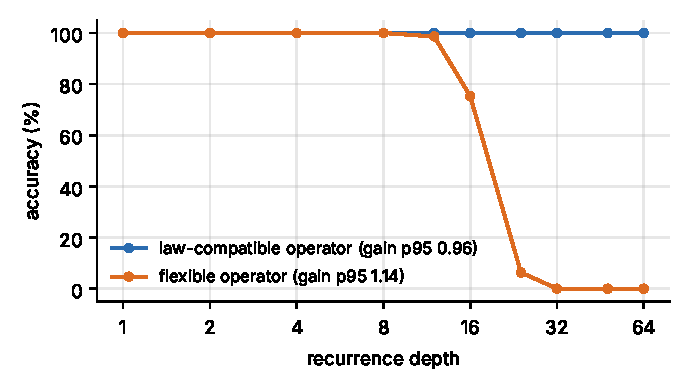
\includegraphics[width=0.62\linewidth]{figures/fig_onestep_vs_recurrent.pdf}
\caption{Two operators with perfect one-step accuracy. The one with transverse gain above one
accumulates error and collapses; the one with gain below one is stable.}\label{fig:onestep}
\end{figure}

\subsection{Terminal supervision does not identify the latent state}

\begin{proposition}[periodic gauge]\label{prop:gauge}
Let $G$ be an invertible map of the state space that commutes with every $F_c$ and preserves the
code set. If the loss constrains $D(h_s)$ only for depths $s\in S$, then the systems $T$ and $G\circ
T$ are indistinguishable whenever $\mathrm{ord}(G)\mid\gcd(S)$. If instead the loss constrains
$D(h_t)$ at every depth with one read-out $D$ injective on codes, then $G$ fixes every code.
\end{proposition}
\begin{proof}
Commutation gives $(G\circ T)^s=G^sT^s$, which equals $T^s$ for all $s\in S$ iff
$\mathrm{ord}(G)\mid s$ for all $s\in S$. With a shared read-out at depth one,
$D(Gm_i)=D(m_i)$ for all $i$, and injectivity gives $Gm_i=m_i$.
\end{proof}

We built this degeneracy explicitly in a recurrent lookup. With supervision only at depth 2,
three runs converge to $G\approx-I$: odd depths have $0\%$ canonical accuracy with cosine $-1$
while even depths are exact. With supervision only at depth 3, intermediate states cycle with
cosines $-\tfrac12,-\tfrac12,1$. Supervising depths $\{2,3\}$ ($\gcd=1$) removes the ambiguity
and every intermediate state becomes canonical. A far-initialized $\{2,3\}$ run still converges
to a non-zero-loss basin: removing an exact degeneracy does not make optimization benign. Per-step
read-out heads $D_t$ would reintroduce the gauge as $D_t=D\circ G^{-t}$; this is why the latent
loops below use a single shared read-out.

\subsection{Reuse the carrier, not the query}

In key--value retrieval, a protected carrier $a_i(q)=\mathrm{softmax}_i(\beta\cos(Qq,Kk_i))$,
$p(q)=\sum_ia_i(q)v_i$, copies the payload without a learned output rotation, so the payload
coordinate system is preserved. In a 10M-parameter token model this gives $4032/4032$ exact
lookups on the locked test in three seeds, with zero, deranged and query-cyclic controls at
$0/4032$. Feeding back the carrier, $q_{t+1}=p_t$, instead of the original query turns one-hop
lookup into composition of unseen permutations: trained on depths 1--4, the locked test is exact
through depth 16 and an exploratory run is exact through depth 64; corrupting the state after
hop 2 drops later accuracy to about $15\%$. The soft state does not converge to a one-hot code:
with eight orthogonal codes, the dynamics settle on a symmetric fixed point with correct-address
mass $a^*\approx0.510$ and cosine $0.940$ to the target. A continuous attractor basin, not
discreteness, is what keeps the loop valid. Section~\ref{sec:capture} turns this observation into a
design principle.

\subsection{Generated values can be reused}

Retrieval is not computation if the next state already exists as a payload. In a modular
arithmetic task, an operator fitted only on one-step pairs must generate a new value, which is
fed back without snapping. Every transition used at evaluation comes from the held-out pair
split. In an operator-compatible Fourier chart with a local bilinear law, accuracy is $100\%$ at
depths $1,2,4,8,16,32$ in three split seeds, while a more general bilinear operator with good
one-step held-out accuracy collapses almost immediately under feedback. Geometry and operator
family must be chosen together.

\section{Attractor capture}\label{sec:capture}

Consider the captured loop $h_{t+1}=\Pi(F_{c_t}(h_t))$, where $\Pi$ is a clean-up map. $\Pi=\mathrm{id}$
is plain continuous feedback; $\Pi=$ nearest-code snapping is a discrete executor. Assume that on
$B(m_j,Lr+\varepsilon)$ the map $\Pi$ is $\kappa$-Lipschitz and that $\norm{\Pi(m_j)-m_j}\le\eta$.

\begin{theorem}[tube invariance]\label{thm:tube}
If $\kappa(Lr+\varepsilon)+\eta\le r$, then $h_0\in B(m_{i_0},r)$ implies $h_t\in B(m_{i_t},r)$
for all $t$ and every instruction sequence. If moreover $r<\rho$, decoding is exact at every
depth. A radius $r$ satisfying the condition exists iff $\kappa L<1$, and the smallest is
$r^*=(\kappa\varepsilon+\eta)/(1-\kappa L)$.
\end{theorem}
\begin{proof}
$\norm{F(h)-m_{P(i)}}\le\norm{F(h)-F(m_i)}+\varepsilon\le Lr+\varepsilon$, so
$\norm{\Pi(F(h))-m_{P(i)}}\le\kappa(Lr+\varepsilon)+\eta\le r$. Induct on $t$. The condition is
affine in $r$ with slope $\kappa L-1$.
\end{proof}

With $\Pi=\mathrm{id}$ ($\kappa=1,\eta=0$) this reduces to Lemma~\ref{lem:acc}: stability needs
$L<1$. Capture replaces it with $L<1/\kappa$.

\begin{proposition}[sharpness]\label{prop:sharp}
For $F(h)=m'+L(h-m)+\varepsilon u$ and $\Pi(y)=m'+\kappa(y-m')$ with unit $u$, the error obeys
$e_{t+1}=\kappa(Le_t+\varepsilon)$. It is bounded iff $\kappa L<1$; it grows linearly at
$\kappa L=1$ and geometrically above.
\end{proposition}

\paragraph{Hopfield capture.} Let $\Pi_\beta(y)=\sum_j p_j(y)m_j$ with
$p(y)=\mathrm{softmax}(\beta\ip{y}{m_j})_j$, a single attention step over the code book.

\begin{lemma}[capture]\label{lem:capture}
For $y\in B(m_i,s)$ with $s<\Delta/(2R_0)$, let $\delta=(N-1)e^{-\beta(\Delta-2R_0s)}$. Then
$1-p_i(y)\le\delta$, $\ \norm{\Pi_\beta(y)-m_i}\le2R_0\delta$, and
$\norm{\partial\Pi_\beta/\partial y}\le4\beta R_0^2\delta$.
\end{lemma}
\begin{proof}
For $j\ne i$, $\ip{y}{m_i-m_j}=\ip{m_i}{m_i-m_j}+\ip{y-m_i}{m_i-m_j}\ge\Delta-2R_0s$, so
$p_j/p_i\le e^{-\beta(\Delta-2R_0s)}$ and $1-p_i\le\delta$. Next,
$\Pi_\beta(y)-m_i=\sum_{j\ne i}p_j(m_j-m_i)$ has norm at most $2R_0(1-p_i)$. Finally, the
Jacobian is $\beta\,\mathrm{Cov}_p(m)\preceq\beta\sum_jp_j(m_j-m_i)(m_j-m_i)^\top$, whose norm
is at most $4\beta R_0^2(1-p_i)$.
\end{proof}

\begin{theorem}[Hopfield capture tolerates any gain]\label{thm:hopfield}
Let $\bar L=\max(L,1)$. If $\varepsilon<\Delta/(2R_0)$, then for every $\beta\ge\beta^*$ with
\[
\beta^*=\min_{s\in(\varepsilon,\,\Delta/2R_0)}\ \frac{\ln\!\big(2R_0\bar L(N-1)/(s-\varepsilon)\big)}{\Delta-2R_0s},
\]
the loop $h\leftarrow\Pi_\beta(F_c(h))$ decodes exactly at every depth from any start in
$B(m_{i_0},(s-\varepsilon)/\bar L)$.
\end{theorem}
\begin{proof}
Let $r=(s-\varepsilon)/\bar L\le s$. $F_c$ maps $B(m_i,r)$ into $B(m_{P_c(i)},s)$. By
Lemma~\ref{lem:capture}, $\Pi_\beta$ maps that ball into $B(m_{P_c(i)},2R_0(N-1)e^{-\beta(\Delta-2R_0s)})$,
which lies in $B(m_{P_c(i)},r)$ once $\beta\ge\beta^*$. Since $r\le s<\Delta/(2R_0)\le\rho$
(because $\Delta\le2R_0^2$), decoding is exact.
\end{proof}

\paragraph{Consequences.}
(i)~The only per-step requirement on the learned transition is a closure defect below
$\Delta/(2R_0)$ (for orthogonal codes, $R_0/2$). One-step accuracy with a margin then implies
validity at unbounded depth, which is exactly what fails without capture.
(ii)~Discrete execution is the limit $\beta\to\infty$; a finite temperature suffices, so the loop
stays differentiable. By Lemma~\ref{lem:capture} the Jacobian of $\Pi_\beta$ is exponentially
small near codes, so large $\beta$ also starves learning; annealing $\beta$ upward towards
$\beta^*$ is the natural schedule.
(iii)~\emph{Under-sharp capture is harmful}: for small $\beta$, $\eta=\norm{\Pi_\beta(m_j)-m_j}$ is
large and $\Pi_\beta$ pulls states toward the code mean. We observe this directly in
\S\ref{sec:exp-capture}.

\begin{proposition}[soft routing is absorbed]\label{prop:routing}
If the model mixes transitions, $F=\sum_k\pi_kF_k$ with weights independent of $h$,
$\pi_{k^*}\ge1-\delta_r$ and
$\norm{F_k(m_i)}\le R'$, then $F$ has closure defect at most $\varepsilon+2R'\delta_r$ relative to
$P_{k^*}$ and gain at most $\max_kL_k$. Theorem~\ref{thm:hopfield} applies whenever
$\varepsilon+2R'\delta_r<\Delta/(2R_0)$.
\end{proposition}
\begin{proof}
$F(m_i)-F_{k^*}(m_i)=\sum_{k\ne k^*}\pi_k(F_k(m_i)-F_{k^*}(m_i))$ has norm at most
$2R'\delta_r$; the gain bound follows from convexity of the norm.
\end{proof}

A convex mixture of individually valid operators is generally not a valid operator, which is a
known source of drift in soft mixtures. Proposition~\ref{prop:routing} shows that hard
straight-through selection is unnecessary when the state loop contains capture: the model's
ordinary soft attention can pick the operation.

\section{Width: a linear obstruction and how capture evades it}\label{sec:width}

\begin{definition}
Let a grammar group $\mathcal G$ act on a finite state set $X$, $|X|=N$. A \emph{point-separating
exact linear register} is an injective $E:X\to\R^d$ with a representation
$\varrho:\mathcal G\to GL(d,\R)$ such that $E(g\cdot x)=\varrho(g)E(x)$.
\end{definition}

\begin{theorem}[width]\label{thm:width}
If $\mathcal G$ acts 2-transitively on $X$, every point-separating exact linear register has
$d\ge N-1$. In particular, for the affine grammar on $\F_p$ generated by $x\mapsto x+1$ and
$x\mapsto gx$ ($g$ primitive), $d\ge p-1$.
\end{theorem}
\begin{proof}
Let $V=\R^X$ be the permutation module and $L:V\to\R^d$, $e_x\mapsto E(x)$; $L$ is
$\mathcal G$-equivariant. $V=\mathbf 1\oplus W$ with $W$ the zero-sum subspace. For a
2-transitive action the permutation character is $1+\chi$ with $\chi$ irreducible~\cite{serre},
so $W\otimes\mathbb C$ and hence $W$ are irreducible. $\ker L\cap W$ is invariant, hence $0$ or
$W$. If it were $W$, then $L(e_x-e_y)=0$ and $E(x)=E(y)$ for all $x,y$, contradicting injectivity.
So $L$ is injective on $W$ and $d\ge N-1$. The affine group of $\F_p$ is 2-transitive.
\end{proof}

\begin{theorem}[no simultaneous diagonal chart]\label{thm:nodiag}
If $\mathcal G$ acts faithfully on $X$ and is non-abelian, no point-separating exact linear
register admits a basis in which all $\varrho(g)$ are diagonal.
\end{theorem}
\begin{proof}
Simultaneously diagonal matrices commute, so $\varrho([g,h])=I$ and $E([g,h]x)=E(x)$ for all
$x$. Injectivity makes $[g,h]$ act trivially; faithfulness makes $[g,h]=e$ for all $g,h$.
\end{proof}

For the affine grammar over $\F_{31}$, Theorem~\ref{thm:width} predicts $d\ge30$. When we
learn 31 identity codes and only the two generator actions with centered, isotropic geometry,
widths 16, 24, 28 and 29 reach $100\%$ on both trained generators yet stay near chance on
generated mixed programs, while $d=30$ is exact in all six seeds (Figure~\ref{fig:linwidth}).
Non-commutation does not, however, force separate charts: in the full additive-character basis,
addition acts as a local complex product and multiplication as an operand-conditioned
permutation of frequencies, and random mixed programs remain exact through depth 256 in one
shared chart. Globality is possible; it costs width and operator complexity.

\begin{figure}[t]\centering
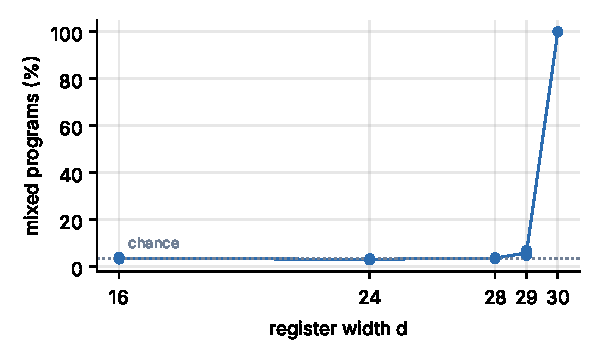
\includegraphics[width=0.52\linewidth]{figures/fig_linear_width.pdf}
\caption{Learned linear register for the affine grammar over $\F_{31}$. Local generator fit is
perfect at every width, but the generated grammar is exact only at $d=30=p-1$.}\label{fig:linwidth}
\end{figure}

The obstruction concerns \emph{exact linear} registers. A captured loop needs only
$\varepsilon$-closure on $N$ points and may be nonlinear, so the bound does not apply.

\begin{proposition}[width--sharpness trade-off]\label{prop:tradeoff}
Equally spaced codes on a circle in $\R^2$ have
\[\Delta=R_0^2\big(1-\cos(2\pi/N)\big)\approx2\pi^2R_0^2/N^2.\]
For well-separated codes on $S^{d-1}$ the gap
scales as $\Delta\asymp R_0^2N^{-2/(d-1)}$, and the regular simplex ($d\ge N-1$) gives $\Delta=R_0^2N/(N-1)$. Theorem~\ref{thm:hopfield} then gives
\[
\beta^*\asymp\frac{\ln(\bar LN)}{\Delta}\asymp\frac{N^{2/(d-1)}\ln(\bar LN)}{R_0^2}.
\]
Exact all-depth recurrence of any grammar on $N$ states is therefore possible at $d=2$, paid for in
inverse temperature rather than width.
\end{proposition}

\section{Experiments on capture}\label{sec:exp-capture}

\subsection{Capture rescues learned flexible operators}

The affine grammar over $\F_{31}$ is used with random unit codes in $\R^{32}$. A two-hidden-layer
MLP $F(h,\mathrm{op})$ is fitted on all 62 one-step pairs, with or without input noise $0.05$.
Every run is $100\%$ one-step exact, but the measured local gain is $L=1.8$--$4.2$
(Table~\ref{tab:rescue}). Without capture, depth-256 accuracy is $0$--$54\%$. With Hopfield
capture at $\beta=64\ge\beta^*$ every run is exact at depth 256 (Figure~\ref{fig:rescue}). At
$\beta=4$ the loop collapses by depth 8: $\beta=4$ is far below $\beta^*$ and $\eta$ is large.
$\beta=16$, below the conservative $\beta^*\approx21$--$33$, is already exact.

\begin{table}[t]\centering\small
\begin{tabular}{@{}lcccccc@{}}\toprule
run & $\varepsilon$ & $L$ & $\beta^*$ & no capture & $\beta=4$ & $\beta=64$\\\midrule
seed 0, clean & 0.020 & 3.82 & 22.1 & 0\% & 0\% & \textbf{100\%}\\
seed 1, clean & 0.013 & 4.00 & 23.2 & 0\% & 0\% & \textbf{100\%}\\
seed 2, clean & 0.004 & 4.16 & 21.0 & 0\% & 0\% & \textbf{100\%}\\
seed 0, noise 0.05 & 0.083 & 1.78 & 28.9 & 53.5\% & 0\% & \textbf{100\%}\\
seed 1, noise 0.05 & 0.084 & 1.89 & 32.7 & 4.3\% & 0\% & \textbf{100\%}\\
seed 2, noise 0.05 & 0.082 & 1.86 & 29.5 & 29.7\% & 0\% & \textbf{100\%}\\\bottomrule
\end{tabular}
\caption{Learned flexible operators, $d=32$, $\Delta\approx0.47$--$0.50$. Depth-256 exact-trajectory rate over 512 random programs.}\label{tab:rescue}
\end{table}

\begin{figure}[t]\centering
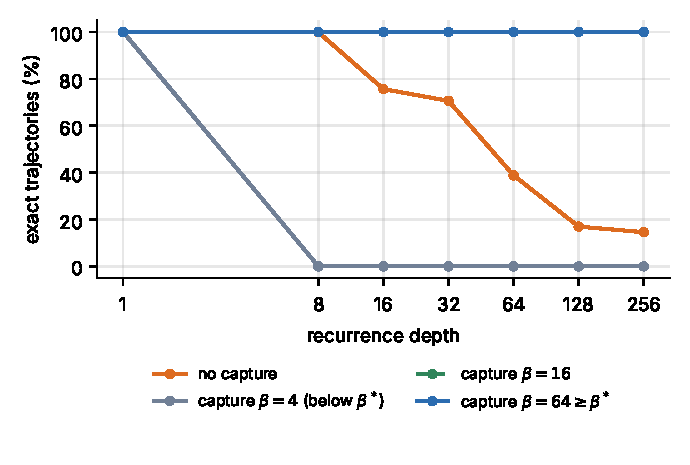
\includegraphics[width=0.62\linewidth]{figures/fig_capture_rescue.pdf}
\caption{Mean over the six runs of Table~\ref{tab:rescue}. Continuous capture at sufficient
$\beta$ turns a drifting learned operator into an exact one at depth 256 (the $\beta=16$ curve
coincides with $\beta=64$).}\label{fig:rescue}
\end{figure}

\subsection{Width--sharpness trade-off with learned operators}

For $d\in\{2,3,4,8,16,32\}$ we place 31 codes on $S^{d-1}$ (regular polygon for $d=2$, otherwise
repulsion minimizing the maximal cosine), fit the MLP on the 62 one-step pairs, and sweep
$\beta$ over $2^{k/2}$, $k=0,\dots,26$. Table~\ref{tab:width} and Figure~\ref{fig:tradeoff}
summarize three seeds per width.

\begin{table}[t]\centering\small
\begin{tabular}{@{}rcccccc@{}}\toprule
$d$ & $\Delta$ & $L$ & smallest exact $\beta$ & $\beta^*$ (theory) & no capture & $\beta\ge\beta^*$\\\midrule
2 & 0.021 & 3.8--4.5 & 181 & 768--841 & 0/3 & 3/3\\
3 & 0.195--0.201 & 5.7--7.5 & 22.6 & 59--60 & 0/3 & 3/3\\
4 & 0.389--0.398 & 3.8--4.1 & 11.3--16 & 26--27 & 0/3 & 3/3\\
8 & 0.744--0.758 & 2.6--2.9 & 8 & 12.2--12.6 & 0/3 & 3/3\\
16 & 1.000 & 1.9--2.1 & 8 & 8.6--8.7 & 0/3 & 3/3\\
32 & 1.033 & 1.4--1.5 & 8 & 7.9--8.0 & 3/3 & 3/3\\\bottomrule
\end{tabular}
\caption{Depth-256 exactness. The repulsion at $d=32$ recovers the regular simplex,
$\Delta=31/30$. No run fails at any $\beta\ge\beta^*$ ($18\times27$ cells), and
$\beta_{\mathrm{emp}}\Delta$ stays within $3.7$--$8.3$ over a fifty-fold range of $\Delta$.}\label{tab:width}
\end{table}

\begin{figure}[t]\centering
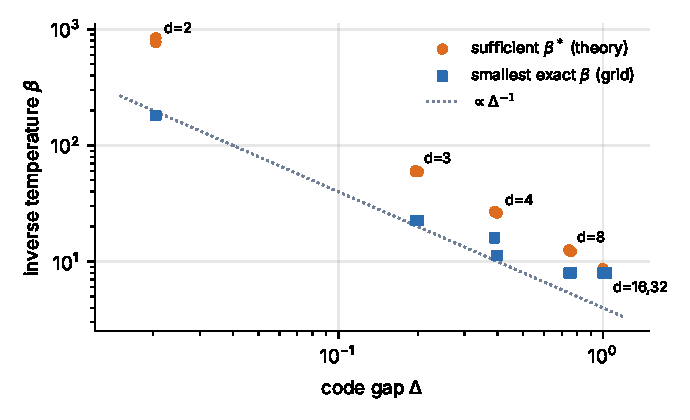
\includegraphics[width=0.62\linewidth]{figures/fig_width_sharpness.pdf}
\caption{Inverse temperature needed for exact depth-256 recurrence versus the code gap.
Both the sufficient bound and the empirical threshold follow $\Delta^{-1}$. A two-dimensional
register suffices for the affine grammar over $\F_{31}$, at $\beta\approx181$.}\label{fig:tradeoff}
\end{figure}

Two observations go beyond the theorem. First, width itself buys stability: at $d=32$ the
fitted operator has $L\approx1.4$ but is exact at depth 256 even without capture, consistent with
the large gap leaving room for errors to stay inside the decoding region. Second, at $d=32$
capture with $\beta\le5.7$ breaks this uncaptured success: under-sharp capture is worse than none,
as predicted by consequence~(iii).

\subsection{Measuring gain at language-model width}

Full $d\times d$ Jacobians are impractical at model width. Randomized Jacobian--vector products
recover the quantities used above: we validated JVP-based relation and gain probing at widths
128, 256 and 320 through a transformer recurrent transition. One implementation detail matters:
CPU flash scaled-dot-product attention does not support forward-mode AD, so probes must use the
math attention backend while ordinary inference is unchanged.

\subsection{Where to read the state in a pretrained LLM}\label{sec:probe}

A latent loop must decide which hidden state to feed back. We probed every layer of a frozen
SmolLM2-135M-Instruct (30 layers, width 576) on natural-language modular-arithmetic programs
(``Work modulo 31. Start with 17. Step 1: Add 8. \dots''), with independent train, validation
and test sets. At the final layer the starting value is linearly decodable at $100\%$ but the
operation identity only at $51.9\%$. At layer 18 the operation is decodable at $100\%$ (layer 17:
$99.3\%$) while the value is still $94.3\%$. The information needed to choose the next operation
peaks mid-stack and is partly mixed away by the output. Feeding back the final hidden state, as
in Coconut-style loops, may therefore discard exactly the control information the next step
needs. This is one model on one synthetic task; it motivates prediction P4 below. For reference,
the same model answering by ordinary generation solves only $0$--$12\%$ of these programs at
depths 1--12.

\subsection{Pilot: a latent loop inside the LLM}

We ran a latent loop with no external executor. The prompt is encoded once by the frozen model.
Each latent step appends the marker tokens `` Step $t$:'' and one latent input vector $x_t$; a
rank-8 LoRA is active only on these thought positions (2.8M trainable parameters including
read-out and codes). The last hidden state
$h_t$ is decoded by one shared linear read-out $D$, supervised with the intermediate value; step 0
reads the starting value. Feedback is either continuous, $x_{t+1}=\mathrm{rescale}(Wh_t)$, or
captured, $x_{t+1}=\sum_v\mathrm{softmax}(\beta D(h_t))_vc_v$ over learned codes $c_v$ ($\beta=1$ on
learned logits, so the effective sharpness is learned), or a
straight-through snap as a discrete reference. Training used 900 CPU steps with batch 16 and a depth
curriculum $1\to4$.

\begin{table}[t]\centering\small
\begin{tabular}{@{}lcccc@{}}\toprule
feedback & $R=1$ (train/new style) & $R=2$ & $R=3$ & $R\in\{4,5,6,8\}$ mean\\\midrule
continuous & 52/54\% & 21/17\% & 8/6\% & 4.2\%\\
capture ($\beta=1$) & 63/63\% & 8/8\% & 0/6\% & 2.9\%\\
snap (reference) & 42/50\% & 19/8\% & 2/8\% & 3.9\%\\\bottomrule
\end{tabular}
\caption{Pilot latent loop in SmolLM2-135M, 48 programs per cell, chance $3.2\%$.}\label{tab:pilot}
\end{table}

\textbf{The pilot is inconclusive} (Table~\ref{tab:pilot}). The loop learned to read the start
value: in the capture arm the fed-back state after step 0 lies within about $1\%$ (relative norm)
of the correct code on average. It reached only $42$--$63\%$ accuracy after one operation, so $\varepsilon\gg\Delta/(2R_0)$
and the hypothesis of Theorem~\ref{thm:hopfield} is not met. In this regime capture locks onto
wrong codes: the mean relative distance to the correct code rises to about $0.98$, against
$\approx1.41$ for an orthogonal wrong code, so most later states sit on wrong codes.
The pilot neither supports nor refutes capture in language models; it shows that one-step
closure must be reached first.

\section{Predictions for latent-reasoning language models}\label{sec:predictions}

\begin{description}[leftmargin=1.2em,itemsep=2pt]
\item[P1 (gain predicts erosion).] For a latent-reasoning model, estimate $\hat\varepsilon$ and
$\hat L$ of the map $h_t\mapsto h_{t+1}$ by JVPs. Across checkpoints and tasks, the depth at which
accuracy starts to erode should increase with $1/\hat L$ and with $1/\hat\varepsilon$, and should not
precede the guarantee horizon of Lemma~\ref{lem:acc}.
\item[P2 (capture flattens depth curves).] Inserting $\Pi_\beta$ over a code book of
task-relevant states (learned codes or token embeddings) with $\beta$ above an estimate of
$\beta^*$ should flatten accuracy versus number of latent steps. $\beta$ well below it should
hurt (consequence~iii).
\item[P3 (shared read-out).] Intermediate supervision through one shared read-out should
extrapolate in depth better than per-step heads (Proposition~\ref{prop:gauge}).
\item[P4 (tap depth).] For operation-conditioned loops, feeding back a mid-stack state should beat
feeding back the final hidden state (\S\ref{sec:probe}).
\end{description}

\paragraph{Decisive experiment.} A Coconut-style model with and without capture, matched against
explicit chain-of-thought at equal compute, on a planning task (graph search) and an arithmetic
task, measuring accuracy versus latent steps, $\hat L$, $\hat\varepsilon$ and the distance of fed-back
states to the nearest code. The theory predicts the captured arm extrapolates past the training
depth when, and only when, one-step closure satisfies $\varepsilon<\Delta/(2R_0)$.

\section{Limitations}

\begin{enumerate}[leftmargin=*,itemsep=2pt]
\item The theorems assume a finite code set. Open-ended reasoning states may not be well
described by a fixed code book; capture over a learned or contextual code book is an assumption,
not a result.
\item Theorem~\ref{thm:hopfield} is sufficient, not necessary; the empirical threshold is up to
$4.6\times$ lower for narrow registers and close to the bound for wide ones.
\item The width theorems are about exact linear equivariant registers. They do not bound
approximate, nonlinear or multi-chart solutions.
\item Most evidence is synthetic: modular arithmetic, affine actions and permutation lookup.
\item The only in-LLM experiment is an underpowered pilot. No comparison with explicit
chain-of-thought or published latent-reasoning models has been made yet.
\item Capture trades gradient signal for stability (Lemma~\ref{lem:capture}); how to schedule
$\beta$ during training at scale is open.
\end{enumerate}

\section{Conclusion}

A continuous thought is useful for reasoning only if the next step can consume it. We gave
measurable conditions for this (closure defect, transverse gain, code gap), showed that terminal
supervision cannot certify it, and proved that a single continuous attractor-capture step makes
recurrence exact at every depth for any local gain once one-step closure is below half the
normalized code gap, at a finite and explicit temperature. Discreteness is then a property of
the dynamics, not a separate processor. The same analysis turns the width cost of exact linear
registers into a sharpness cost. Whether these conditions explain and repair the depth erosion of
latent reasoning in language models is the empirical question the predictions above are designed
to settle.

\appendix
\section{Evidence provenance}\label{app:prov}

\begin{center}\small
\begin{tabular}{@{}>{\raggedright\arraybackslash}p{0.3\linewidth}>{\raggedright\arraybackslash}p{0.64\linewidth}@{}}\toprule
claim & artifact / script (repository paths)\\\midrule
one-step vs recurrence, gain diagnostic & \path{artifacts/research/stability_diagnostic/seed22.json}, \path{artifacts/research/exp_014/}; \path{transition_stability_diagnostic.py}\\
periodic gauge & \path{artifacts/research/exp_003/metrics.json}; \path{generated_value_gauge_experiment.py}\\
protected carrier, composition & exact-binding logs under \path{artifacts/}; \path{artifacts/research/exp_001/}; \path{recurrent_binding_composition_experiment.py}\\
generated values & \path{artifacts/research/exp_005/}; \path{learned_generated_value_recurrence_experiment.py}\\
learned linear width threshold & \path{artifacts/research/exp_022/}; \path{isotropic_affine_representation_experiment.py}\\
shared chart for ADD/MUL & \path{artifacts/research/exp_019/}; \path{single_chart_affine_machine_experiment.py}\\
JVP probing at width 320 & \path{artifacts/research/exp_036/}; \path{highdim_jvp_relation_discovery_experiment.py}\\
capture theorem, numeric check & \path{experiments/capture_theorem_check.py}\\
capture rescue (Table~\ref{tab:rescue}) & \path{artifacts/capture-learned-operator/}; \path{experiments/capture_learned_operator_experiment.py}\\
width--sharpness (Table~\ref{tab:width}) & \path{artifacts/capture-width-sharpness/}; \path{experiments/capture_width_sharpness_experiment.py}\\
LLM layer probes & \path{research/PRETRAINED_LLM_RETROFIT_REPORT.md}; \path{experiments/fog_retrofit_smollm135m_layer_sweep.py}\\
pilot latent loop & \path{artifacts/latent-loop-llm/}; \path{experiments/latent_loop_llm_experiment.py}\\
figures & \path{paper/make_figures.py}\\\bottomrule
\end{tabular}
\end{center}

\begin{thebibliography}{99}\small
\bibitem{coconut} S.~Hao, S.~Sukhbaatar, D.~Su, X.~Li, Z.~Hu, J.~Weston, Y.~Tian. Training large language models to reason in a continuous latent space. arXiv:2412.06769, 2024.
\bibitem{quietstar} E.~Zelikman, G.~Harik, Y.~Shao, V.~Jayasiri, N.~Haber, N.~D.~Goodman. Quiet-STaR: Language models can teach themselves to think before speaking. arXiv:2403.09629, 2024.
\bibitem{geiping} J.~Geiping et al. Scaling up test-time compute with latent reasoning: a recurrent depth approach. arXiv:2502.05171, 2025.
\bibitem{looped} Y.~Fan, A.~Svete, K.~Lee. Bridging the gap between latent and explicit reasoning with looped transformers. arXiv:2606.31779, 2026.
\bibitem{softthinking} Z.~Zhang et al. Soft thinking: unlocking the reasoning potential of LLMs in continuous concept space. 2025.
\bibitem{ut} M.~Dehghani, S.~Gouws, O.~Vinyals, J.~Uszkoreit, \L.~Kaiser. Universal Transformers. arXiv:1807.03819, 2018.
\bibitem{act} A.~Graves. Adaptive computation time for recurrent neural networks. arXiv:1603.08983, 2016.
\bibitem{ntm} A.~Graves, G.~Wayne, I.~Danihelka. Neural Turing machines. arXiv:1410.5401, 2014.
\bibitem{hopfield} J.~J.~Hopfield. Neural networks and physical systems with emergent collective computational abilities. PNAS 79(8), 1982.
\bibitem{ramsauer} H.~Ramsauer et al. Hopfield networks is all you need. arXiv:2008.02217, 2020.
\bibitem{plate} T.~A.~Plate. Holographic reduced representations. IEEE Trans.\ Neural Networks 6(3), 1995.
\bibitem{kanerva} P.~Kanerva. Hyperdimensional computing. Cognitive Computation 1(2), 2009.
\bibitem{serre} J.-P.~Serre. Linear Representations of Finite Groups. Springer, 1977.
\end{thebibliography}
\end{document}
